\documentclass[10pt,journal]{IEEEtran} 
\usepackage{graphicx}
\usepackage{listings}

\usepackage{pgfplots}
\pgfplotsset{compat=newest}


\title{A tool for gathering unbiased sets of videos and metadata from YouTube}
\author{
    Kragset, Hans Petter Taugb\o l
    \and
    Wallenburg, Hugo Matthijs Harstad
    \and
    Krieger, Lukas
    \and
    \newline
    \texttt{\{hpkragse, hugomw\}@ifi.uio.no},
    \texttt{lukas.krieger@me.com}
}
\date{\today}

\begin{document}

\maketitle

\begin{abstract}
    YouTube provides a massive amount of media data freely, available as video and
audio data. Analysing this data can provide invaluable information, and YouTube
is especially interesting as there is a similarily massive amount of metadata
available. Analysing video together with metadata such as recording time and
location, view count, like and dislike counts, description, tags and last but
not least comments enables a whole new depth of video analysis. With this in 
mind we have developed a tool that makes it easy to download a set of videos
with related metadata and comments. The tool groups the data in an SQL database.
When downloading data our tool tries to be as unbiased as possible, by
downloading as much data as it can and leaving the query parameters in the users
control. Being unbiased is important because having a representative video set
to, for instance, train a machine learning video analysis algorithm is essential
for that algorithm's ability to understand a video outside of the training set.
During development we discovered interesting aspects about the YouTube API.
The API seems to be inconsistent in the replies it gives, the API endpoint gives
slightly different results when queried with the same query multiple times. This
behaviour is understandible and negligible, and does not compare to the issue
that is the massive dropoff of returned result when stepping backwards in time.
Compared to requesting videos from yesterday, requesting videos form a day a
months back return only about 2\% of the unique video ID count. 

YouTube uses Dynamic Adaptive Streaming over HTTP, DASH, to provide it's media
content. Our tool uses this to provide the user with information about available
qualities for a given video or video query set, and subsequently issues HTTP GET
requests as described in the DASH Media Presentation Description (MPD). 
YouTube's implementation of DASH does not differ much from ISO 23009-1 where 
DASH is defined.

\end{abstract}

\begin{IEEEkeywords}
    MPEG-DASH, YouTube, Metadata, unbiased dataset
\end{IEEEkeywords}

% About YouTube
%	Short description
%	Why one would want an unbiased dataset
%		What does "unbiased" mean in this context
%		How have we interpreted this, and how has it affected our work?
% Our tool
%	Short description
%	How we select videos
%	User choices in request vs. biased selection
%	API over crawling
% Sections

\section{Introduction}

YouTube is without a doubt the world's largest host of user-generated content,
with over one billion users generating several billion views, spending hundreds
of billions of hours every day ~\cite{officialstats}. Though there does not seem
to be an official source, it is believed that by the end of 2014, more than 300
hours worth of content was being uploaded to YouTube every minute 
~\cite{dagensmediastats}~\cite{reelseostats}. 

This makes YouTube a fantastic resource of both videos and metadata to be used
for analysis for a range of different purposes. Especially with regards to
machine learning algorithms, a large, good sample set of videos will be required
to train an algorithm. For such an algorithm to stay relevant also for videos
that was not in the inital training set, the training set will have to be as
unbiased as possible.

It is neither our desire nor task to create a tool that by default limits the
returned data set in any way. By letting the users specify as little or as much
as they want in their query, we leave as much control as possible with the user,
who, of course, knows much better than us what the resulting dataset will be
used for. This makes the tool very versatile, as you could, for instance, first
download a big set of videos related to the search term "cat", before
downloading a completely random video set and using an algorithm trained with
the first data set to find cat-related videos in this second set. 

More specifically, we provide the means to: build a large database of video ID's
\footnote{We fetch as much data as possible within the restraints imposed
on us by the API.}; fetch most metadata\footnote{We fetch all data associated
with a video, as well as its comment threads and replies. Fetching of related
videos has been deliberately left out - for now at least} for the given videos;
fetch the videos themselves, with sound; and connect all related data points
with a SQL database. Alongside the documentation for the source code there will
be a databse diagram show how all the data is related. Making an SQL database
made sense because, as we saw our dataset grow with hundreds of thousands of
videos with related metadata and comment data, storing it in CSV, XML or some
other file format made little sense. SQL is also a widely adapted database
format, and all the widely adapted programming languages has support for
extracting data from an SQL database in one way or another.

One of the main goals of the tool, as described earlier and in even more detail
later, is to be unbiased. In the context of this paper, to be unbiased means
to not whiegh videos differently based on their properties. When gathering a
set of videos, the only limitations, if any, are the ones provided by the user.
The resulting videoset will consist of all videos matching the query, without
being wheighted towards popular videos, new videos, high quality videos, 
advertised videos, recommended videos or any other imaginable parameter. This
is inherently different from the video set a normal user sees while browsing, 
and this is discussed later.

With this foundation our work has been centered around trying to gather as much
information as possible from YouTube whilst being unbiased and efficient with
resources. Resources can here mean several things, as well as the users CPU,
network and storage resources, we also have tried minimising the API quota
\footnote{A form of cradit assosiated with an API key, quota is lost when making
API requests.} costs for the user.



\section{Related Work}
A lot of work has by now been done related to DASH and Adaptive streaming in
general. DASH~\cite{iso-dash-2014} was the first adaptive streaming
technology using HTTP that became an international standard. This is in large
due to pioneering work from Adobe with their Adobe Systems HTTP Dynamic
Streaming~\cite{adobe-http-dynamic-streaming}, Apple with HTTP Live Streaming
(HLS)~\cite{apple-http-streaming}, and Microsoft with Microsoft Smooth
Streaming~\cite{microsoft-smooth-streaming}, DASH has quickly spread, and
YouTube has now implemented DASH as their preferred streaming
technology~\cite{Google I/O 2013}. 
D. Krishnappa et al. (2013)~\cite{dashing-youtube} discussed possible resource
savings of implementing DASH in YouTube, somewhat related to our work. 

youtube-dl (sic)~\cite{youtube-dl} is an open source tool developed by P.
Hagemeister et al. (2008-today) that provides the ability to download videos
from YouTube and other similar media hosting sites. Their source code has been
the only significant inspiration for our own source code. We had the option of
simply including their source code and interact with it directly, as a way to
outsource the video file downloading, but the code required is not complex
enough to justify the loss of control. One of the most usable features
youtube-dl provides, that our tool currently does not provide, is the merging of
sound and video into a single file. This would make storage on our part a bit
less complicated, but on the other hand having split video and sound files can
be an advantage for analysis tools. 


\section{DASH}

\subsection{Overview}

Dynamic Adaptive Streaming over HTTP (DASH) is a protocol, defined in
ISO/IEC 23009-1~\cite{iso-dash-2014}, that facilitates 
streaming of multimedia over the internet in varying network conditions.
The goal of DASH is to improve the user
experience while streaming media content by splitting the media file in question
into smaller parts and letting the streaming client choose between several
different versions of the same file depending on preferred quality and network
conditions. In effect, it allows streaming clients the ability to aggressively
limit stalling in video playback at the cost of perceived video/audio quality.

The core of DASH is the Media Presentation Description (MPD), sometimes
referred to as the DASH manifest. The MPD contains all the information
needed to display the media. When a user wants to access a streamed
media, for instance a video, the streaming client (or website frontend)
makes a request to get the MPD for the requested media. The client then
parses the MPD and meassures available network and buffer resources,
before the streaming is commenced at the best feasable quality. Many clients %TODO: references?
seem to prefer starting the stream at the lowest available quality, and
slowly ramp the quality up if no network problems occur. The
client continues to monitor the available resources during playback, adapting
quality dynamically if conditions should change.

With this approach all decisions about download speed are left to the client
alone.
The server simply presents the entirety of the media information in the MPD,
allowing the client to make its own informed choices. The client may choose
to focus on continuous playback, for instance by downloading lower quality
segments during heavy network congestion or local processor load, or it may
force playback of a set quality no matter the conditions under which it
operates. The behavioral pattern for most media streaming clients, among
others YouTube's own media player, seems to be to value continuous playback
over intermittent delays in high quality playback, unless the user should want
to force a specific quality setting thus overriding default behavior.

The developed tool only downloads the media files as specified by the
user, and does not care about available resources or the user experience.
The DASH manifest is still parsed, and all relevant data is stored in the
database to provide an overview of the available medias and qualities,
and their respective properties. Although we are not using DASH to
accomplish better user experience, the MPD is still very useful as a
single point to get information about a streamed media.

\subsection{Details}

\begin{figure}
	\centering
	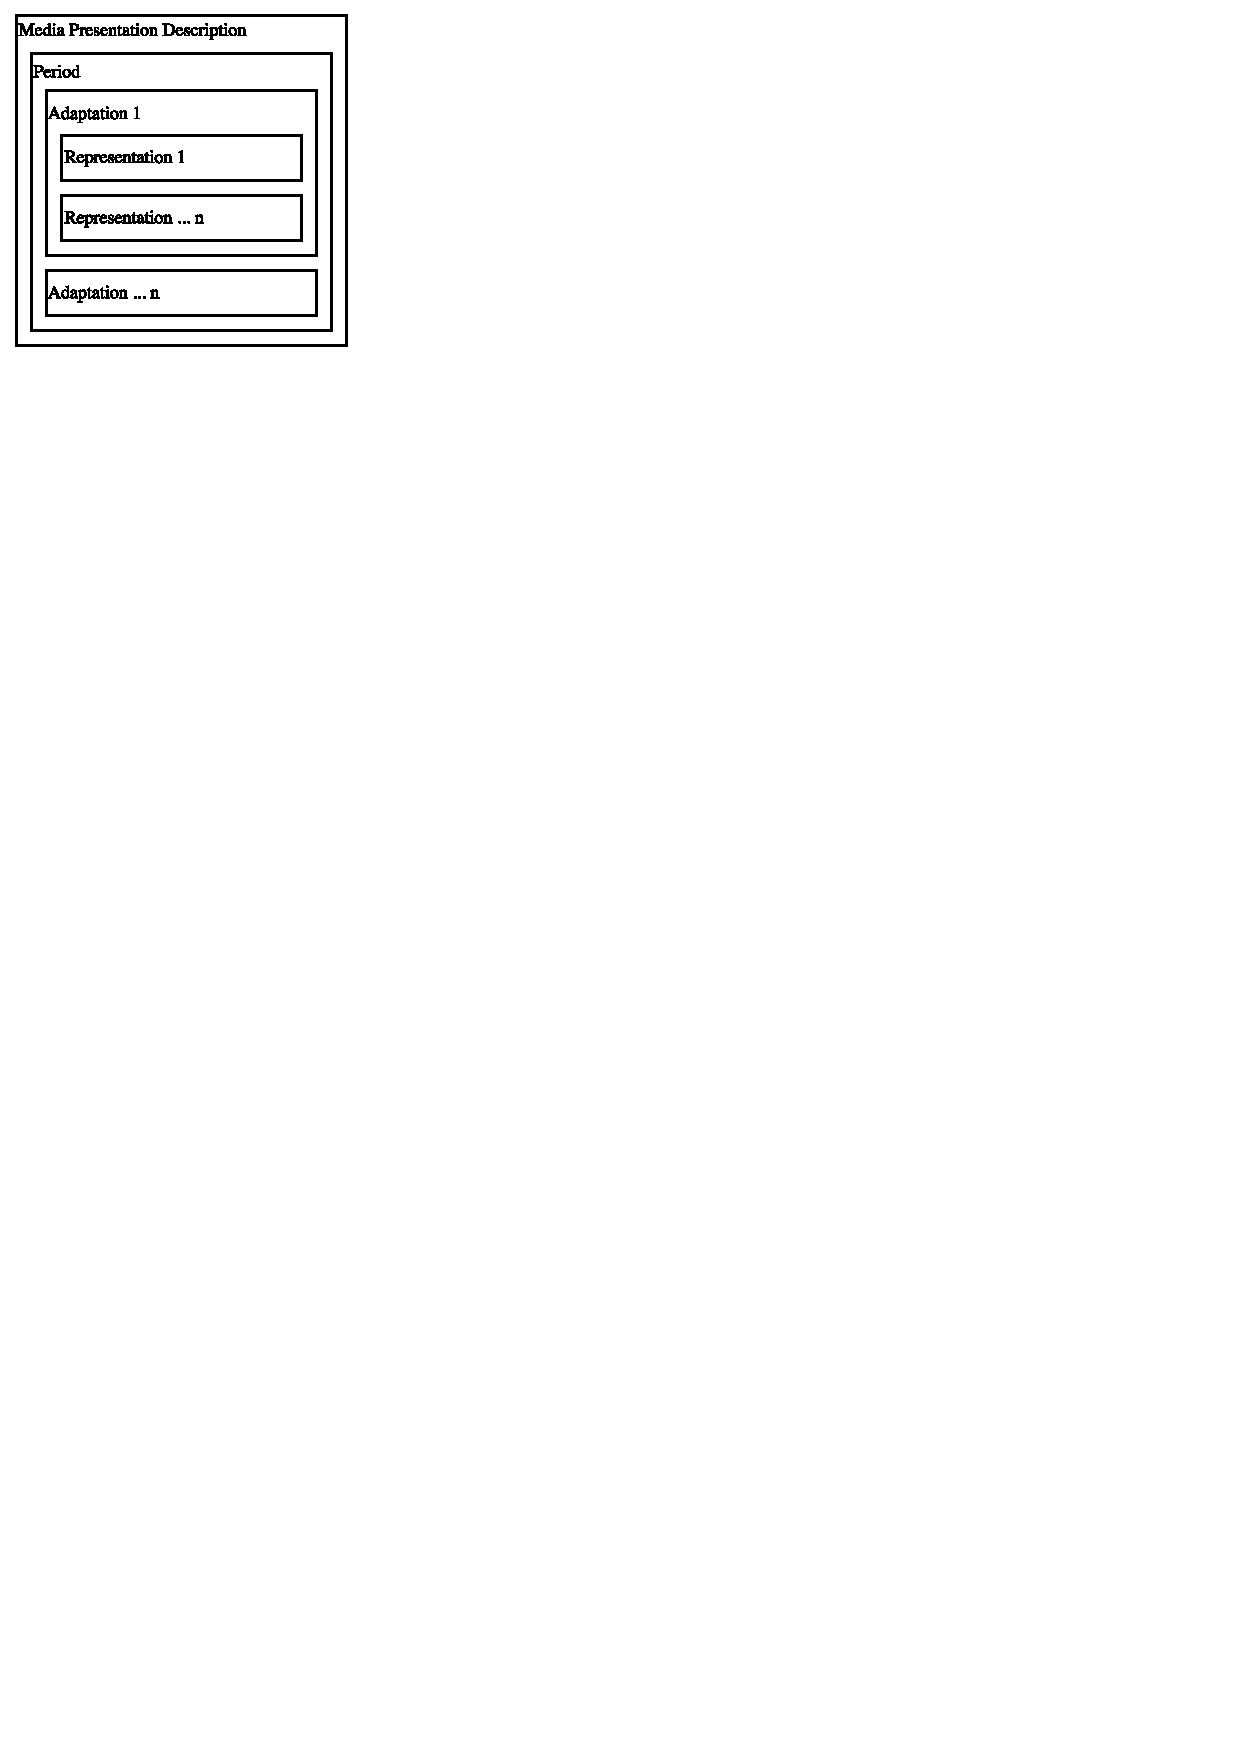
\includegraphics[width=0.2\textwidth]{figures/dash-mpd-diagram}
	\caption{Diagram of the YouTube Media Presentation Description.}
    \label{fig:dash-mpd-diagram}
\end{figure}

~\ref{fig:dash-mpd-diagram} depicts the basic outline of a Media Presentation
Description. The uppermost layer of the YouTube MPD contains duration of the
media as well as information about the format. Each MPD contains a set of
adaptations, each describing a media type. An arbitrary YouTube video might have
the following adaptations: audio/mp4, audio/webm, video/mp4, video/webm. There
are also different adaptations for 3D videos, live media streams, etc. Each
adaptation (media type) might have multiple representations each designating a
different media quality.

Note that this differs from what one might consider the \textit{standard ISO
DASH}\footnote{The DASH standard is incedibly loose in order to allow different
implementations and the freedom to make changes that benefit the specific media
host the most, thus there is not really a \textit{standard} DASH implementation.}
implementation. The standard facilitates using periods to
describe discrete segments within the media, with each period containing links
to separate files containing separate quality versions of that same period.
YouTube works differently: There is only one period, with several adaptations
describing different media types, each with several representations describing
different qualities of media. YouTube MPD representations contain a single file\footnote{Or more specifically, a single URI}
containing the entire video in the quality specified in the representation.
The media player client does not have to do anything more advanced than simply
request this file in order to play the designated media. If it is to utilize
DASH, however, it needs to calculate which chunks of which file it needs to
fetch in order to assure smooth playback.

\begin{figure}
    \centering
    \begin{lstlisting}[
        basicstyle = \footnotesize\ttfamily
    ]
    {
        "@id": "137",
            "@codecs": "avc1.640028",
            "@width": "1920",
            "@height": "1080",
            "@startWithSAP": "1",
            "@maxPlayoutRate": "1",
            "@bandwidth": "4133205",
            "@frameRate": "24",
            "BaseURL": {
                "@yt:contentLength": "148765820",
                "#text": [OMITTED - URI goes here]
            },
            "SegmentBase": {
                "@indexRange": "711-1942",
                "@indexRangeExact": "true",
                "Initialization": {
                    "@range": "0-710"
                }
            }
    }
    \end{lstlisting}
    \caption{Example of a mp4 1080p representation}
    \label{fig:dash-1080p-representation}
\end{figure}

~\ref{fig:dash-1080p-representation} is an example of a Representation of a 1080p mp4 video. The \texttt{@id}
field specifies an identifier for this Representation, it's used to do
what exactly? Each id is linked with a specific type of video. In the case of
YouTube, \texttt{137} is defined to always be a 1920x1080 mp4 video, for
example~\cite[line 303]{youtube-dl:youtube.py}\footnote{The retrieval of MPD's
does not seem to be officially supported in the YouTube API v3, thus there are
no truly reliable sources. The reference is to a popular youtube downloader tool
that seems to have figured out how the MPD is laid out as of 2015-11-01}

The \texttt{@codecs} field shall specify the codecs present with this
Representation. The field should also include the profile and level
information where applicable. For this video, the codec specifies a
H.264/AVC video, High Profile, Level 40 (fix).

The \texttt{@width} and \texttt{@height} fields specifies the resolution of the video in
pixels (not the ISO DASH definition, but always true for youtube
videos?).

TODO: describe SAP

\texttt{@maxPlayoutRate} specifies the maximum playout rate as a multiple of the
regular playout rate, in this example it is set to 1, which means that
it's not supported on any level.

The \texttt{@bandwidth} field is a little more complicated than the other fields.
If a Representation is continuously delivered at this bitrate (in a
constant bitrate channel of \texttt{@bandwidth} bps), starting at SAP 1, a client
can be assured of having enough data for continuous playout providing
playout begins after \texttt{@minBufferTime} * \texttt{@bandwidth} bits have been
received. If you consider the value to be bits per second in a channel
with constant bitrate,

Not all identifiers are specified in the ISO DASH standard. YouTube
provides some of its own, and these are prefixed with yt:. One example
is the \texttt{@yt:contentLength} field. This specifies the size of the
Representation in bytes. So the total download size of the
Representation will match this value.

BaseURL contains the contentLength and a HTTP URL to be used as a base
URL for the Representation.

When switching between different qualities, the base URL is used
together with content length and stuff to start downloading at the
correct loaction for the next Representation. \emph{super pr0
description here}


\section{Architecture}
A client-server model with a REST API was chosen as the tool architecture. The
proposed solution allows the tool to be used by multiple users simultaneously,
as well as enabling deployment to distributed systems with distinct roles,
responsibilities, and hardware resources.
The frontend is a simple thin client whose sole job is relaying commands to a
server and showing the returned results. The server is tasked with obtaining
and processing the available YouTube data, and otherwise interacting with the
API.
Local deployment is a viable option, given sufficient storage and networking
capabilities.


\subsection{Client}
The user interface of the tool is written in AngularJS, an open-source framework
that facilitates easy setup and management of single-page web applications using
the model-view-controller (MVC) pattern.~\cite{architecture:angularjs}

The frontend is separated into four main pages that each have a specific
function: Management of API keys, creation of API queries, creation of celery
tasks, and results presentation.


\subsubsection{User management}


\subsubsection{API key management}
The API key management page lets the user register API keys to his account.
API keys are instantly validated and, if valid, added to the dropdown list of
available keys on the query builder page.
While only a single key is required per API request (in the absence of OAuth
2.0), having access to multiple keys makes for quick and easy testing and the
ability to generate keys for a specific purpose or dataset. The latter is
shown in action on the Result page, where the user can view statistics filtered
by a given API key. %TODO: refine?


\subsubsection{Query Builder}
On the Query builder page the user may build individual search queries using
the provided interface. YouTube's API defines a set of options which we present
to the user in the form of input boxes. Our algorithm for assuring unique
results requires a timeframe, thus the two relevant query fields are required - 
all other fields are deemed optional. Query fields that specify operations
specifically on the user's own videos are deliberately omitted as this is
not within the scope of the tool.

Before queries are dispatched to the task workers and any real work is
performed, they are validated by issuing a small version of the query for
verification only. The user is immediately notified if any of the given query
parameters create an invalid combination. This will prove invaluable to new
users who can safely learn to use the YouTube API, as well as preventing
the storage of invalid queries.
%TODO: reword?


\subsubsection{Task Page}
Stored queries may be executed on the Task page. The user selects the task he
wants performed and a query which defines the set of videos on which to operate.
The first operation will always be the fetching of video IDs, as the rest of the
available tasks depend on this. Multiple tasks may be launched in parallell.
Progress bars are updated in real-time. %TODO: too short and list-y. Reword?


\subsubsection{Result page}
The Result page contains selected statistics for the dataset returned by a given
query. Of particular note is the graph showing the intersection between datasets. This
allows the user to quickly identify closely related queries, and can be helpful
in e.g. parameter studies.
%TODO: Maybe refine a bit.


\subsection{Server}
The server is written in python %TODO: finish


\subsubsection{Background tasks}
All requests created by the frontend are handled asynchronously by Celery and
Redis.

Celery is used as an asynchronous task queue based on distributed messages. It
is capable of distributing tasks over a potentially vast network of nodes.
~\cite{architecture:celery} Redis is a networked in-memory key-value database.
~\cite{architecture:redis} The frameworks aren't used to their full extent given
our current single-server environment, but having these frameworks already
present will be of great aid in future expansion.

After a task has been scheduled by the user, it is immediately pushed to Redis
and put in a pending state until a Celery worker is available to process it.
While the task is executing, Celery provides an interface with which to control
it. It is because of this feature an in-memory database to keep track of running
tasks is preferential. Given that our fetcher modules, the actual tasks that are
being run, update their own status in the database after every single request to
the YouTube API, a disk I/O-bound database would potentially severely limit
performance.


\section{Fetching an unbiased set of video IDs}
For video analysis, an unbiased set of sample videos might be a requirement or
a desire for the analyst. YouTube, of course, is inherently relying on its
ability to provide the users the videos they want, and in turn this leads to
biased samples if one was to simply add the videos one found while
browsing YouTube to a list. To circumvent YouTube's attempts at tailoring a set
of videos, the algorithm uses the API to get videos.

\subsection{The YouTube API}
YouTube provides a REST API, from now on referred to as "the API", which can be
queried for information with a set of parameters. The API consists of different
endpoints, and the one used for searching videos is called "search.list". This
endpoint returns a result as a JSON object. This endpoint provides a rich list
of customizable paramaeters, and optimizing the use of these is important to
achieve high efficiency while using the API. 

For a given query, the search.list response will contain at most 50 videos. There
may be multiple pages, as indicated by a \texttt{nextPageToken} in the JSON
object, but no more than ten pages are returned for any one set of parameters.
To get a complete list of video IDs for a given set of parameters the chosen
query has to be split up into subqueries that by themselves does not match more
than 500 videos. This splitting, and how we recommend doing it, is discussed in
detail in this section.

Why is it important to split up the query into subqueries? The main problem with
the 500 video limit for a static parameter set is that it can not be a good
sample. There might be a lot of other videos which match the requested
parameter, but subsequent requests to the API only return more or less the exact
same sample. There are minor variations in the returned sample, and we will 
discuss this and the related issues in more detail later. 

As a side note it should be mentioned that using an actual web crawler will have
properties an API reliant fetcher can not recreate. A crawler will have its 
behaviour logged by YouTube, which in turn provides more content in line with
what it thinks the crawler likes. The resulting set of videos will be more like
a set of videos a given user is likely to see, it is inherently biased. For some
cases such a set of videos might be desirable, for instance if one wants to
focus on popular videos, or if one wants to measure how biased a set becomes
over time.

Before continuing a few terms will have to be clarified. A  "static parameter 
set" is the set of parameters that are static, globally, for a set of queries, 
like "All videos which are related to the word 'fun', that are 2D and have a 
high video quality". A "variable parameter" is a parameter that can be changed 
for every single request in a request chain, while the static parameter set 
remains untouched. This results in the ability to create many different
variations of the "static parameter set" in order to exceed the 500 videos 
maximum.

From the search.list API endpoint only four different variables can be varied 
between requests in a chain. All other parameters are in some kind static and
would result in a maximum of 500 videos. Following is a description of the
variable parameters.

\subsubsection{location and locationRadius}
The problem with this parameter is that not every video on YouTube has specified
the location in the metadata. Evaluating some hundred thousands of videos
metadata has shown that only 5-10\% of the videos has specified a location in
their metadata. We can not verify that this is the average on all videos
uploaded on YouTube, but just the fact that some (a lot) of videos lack data in
this field indicates that trying to vary it to get an unbiased sample will
result in a set of videos that be default leaves out a lot of videos. For
unbiasedness this is sub-optimal, but not disastrous. It is reasonable to
assume that the set of videos with location data contains a well distributed
and unbiased subset, but this can not easily be verified.

\subsubsection{channelId}
In order to use this parameter as a means of getting an unbiased set of videos,
we would need to have a list of all channels available on YouTube. This is as
difficult as getting all videos of YouTube and therefore varying this parameter 
is probably not a good approach to get an unbiased set of videos. Some channels
also have some thousands of videos uploaded, so with a static parameter set and
only varying the channelId, the API response would be limited to 500 videos. One
could argue that 500 videos is a representative set of videos for a channel, but
the problem is that this subset of the channel's full video list is provided by
YouTube, outside our control. Thus the returned sample can not safely be assumed
to be representative.

\subsubsection{q - search term}
In theory this parameter could be varied and cycled through all possible
combinations of symbols (words, in a wide sense), and through that get an
unbiased set of videos. This is not only unfeasible due to the remarkably big
list of words one would need\footnote{171\,000 words in english alone, then add
all other languages, not to mention names and other word-constructs}, but for
some cases the API quota cost would be extremely high measured as cost per
result. For instance, if one was to get an unbiased set of 3D videos, one would
have to cycle through the whole word list and end up spending quota points on queries
that return stale results. In addition to this, if one is to vary the
search term, the user is left without the ability to manually narrow the result
set. We want to allow the user the ability to create sets of data tailored to
specific tasks, should it be required.

\subsubsection{publishedAfter and publishedBefore}
By having a date range as the varying parameter for a search query, and assuming
that the API actually returns all videos matching the query, the resulting set
would be unbiased with regards to all aspects except from time. Of course, for
a big timeframe there exists more than 500 videos, so to circumvent this cap,
the timeframe can be recursively sliced up until it is so small that less than
500 videos match the parameters. Varying this way leaves the rest of the
parameters unchanged, and the resulting set becomes as much as possible
unbiased.

By slicing the timeframe up like this, one will also be able to get more than
500 videos from a given channel, or from within a geographic zone. It becomes
apparent that varying this parameter alone is the best way to achieve a unbiased
set of videos. A nice bonus is that it also allows customization of the query
without leaving videos out of the resulting set.


\begin{figure}
    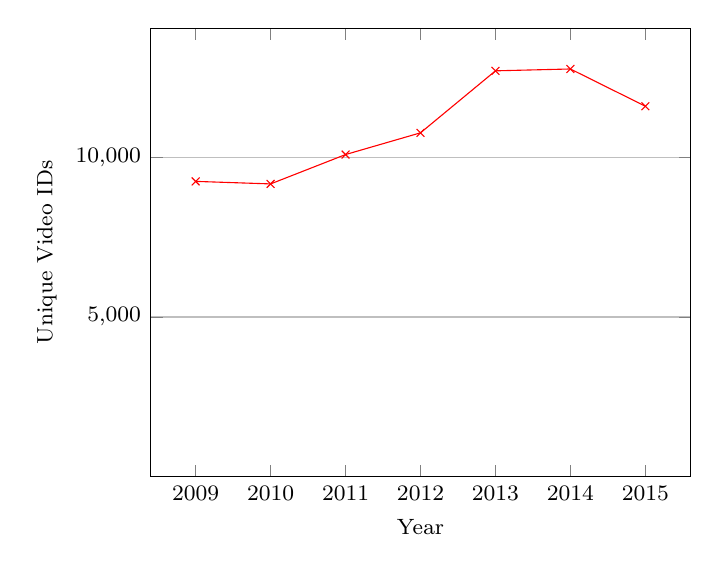
\begin{tikzpicture}
        \begin{axis}[
            ymin = 0,
            xlabel = Year,
            ylabel = Unique Video IDs,
            font = \footnotesize,
            xtick = {1, ..., 7},
            xticklabels = {2009, 2010, 2011, 2012, 2013, 2014, 2015},
            ytick = {5000, 10000},
            scaled y ticks = false,
            ymajorgrids = true
            ]
            \addplot[color=red, mark=x] coordinates {
                (1, 9248)
                (2, 9169)
                (3, 10089)
                (4, 10770)
                (5, 12712)
                (6, 12770)
                (7, 11603)
            };
       %     \addplot[color=blue, mark=*] coordinates {
       %         (1, 8793)
       %         (2, 9180)
       %         (3, 10038)
       %         (4, 8218)
       %         (5, 10205)
       %         (6, 11933)
       %         (7, 11603)
       %     };
        \end{axis}
    \end{tikzpicture}
    \captionof{figure}{Unique video IDs for January, by year [Accessed: 2015-10-31]}
    \label{jan-ids-year}
\end{figure}



\begin{tikzpicture}
	\begin{axis}[
		xlabel=Month,
		ylabel=Unique Video IDs]
	\addplot[color=red,mark=x] coordinates {
		(1,11603)
        (2,11194)
        (3,12907)
        (4,11581)
        (5,11572)
        (6,11609)
        (7,11410)
        (8,12716)
        (9,120304)
        (10,319270)
    };
    \addplot[color=blue,mark=*] coordinates {
        (01,11603)
        (02,11402)
        (03,12905)
        (04,11581)
        (05,11527)
        (06,11640)
        (07,11206)
        (08,12709)
        (09,110822)
        (10,1280155)
    };
	\end{axis}
\end{tikzpicture}


\begin{tikzpicture}[y=.2cm, x=.7cm,font=\sffamily]
 	%axis
	\draw (0,0) -- coordinate (x axis mid) (10,0);
    \draw (0,0) -- coordinate (y axis mid) (0,30);
    %ticks
    \foreach \x in {0,...,10}
    \draw (\x,1pt) -- (\x,-3pt)
        node[anchor=north] {\x};
    \foreach \y in {0,5,...,30}
        \draw (1pt,\y) -- (-3pt,\y);
            node[anchor=east] {\y}; 
	%labels      
	\node[below=0.8cm] at (x axis mid) {Day};
	\node[rotate=90, above=0.8cm] at (y axis mid) {Unique video IDs};

	%plots
	\draw plot[mark=*, mark options={fill=white}] 
		file {video_ids_october.data};    
\end{tikzpicture}



\section{Future work}
Perhaps the most obvious issue to address in future work is the inconsistancy
of the YouTube API. Doing research on what causes inconsistent replies could
initially improve the effectivity of the developed tool, but perhaps more 
importantly it could be used to improve the YouTube API. 

Investigating why the API return rate drops dramatically at certain intervals
when looking back in time, and looking at what kind of videos that disappear
from the returned set, will give interesting knowledge about the YouTube API,
as well as perhaps give a final answer to whether the returned video set is
indeed biased.

There are many conceivable additions to the tool as it is now. Improving the
statistics view could improve the user experience and make it easier for the
user to make decisions about what to do next. A feature that allows the user to
export a database containing only a selected set of videos could drastically
reduce SQL query times during analysis, and we would recommend making some
feature like this if SQL querying becomes a major time and resource consumer.

There is a lot of room for performance improvements, especially when it comes to
concurrency. The tool was tested on a variety of platforms, and performed
reasonably well on most of them, but on certain configurations the API requests
were inexplicably horrendously slow. The cause of this might be a weird
combination of hardware, drivers, and TCP implementation in the OS kernel - 
we simply had no time to narrow down the possible causes. Adding support to run
multiple Celery jobs per task might have alleviated some of the performance
hangups.


\section{Conclusion}
This paper presented how
YouTube distributes it's media content through dynamic streaming over HTTP, and how it
differs from the ISO specification of DASH. It gave an overview of the YouTube
Data API v3, outlined the major limitations of it and also provided some
guidelines on how to bypass these limitations in order to obtain a good sample
of YouTube videos for further analysis. The main decision criteria on
implementing the searching for videos were maximization of the amount of
responded videos while minimizing the quota costs and requests needed to achieve
this, while at the same time trying to maximize resource usage through
concurrency. While creating the tool, there were 2305 open issues associated to
the YouTube API on the Google Data APIs issue tracking
platform~\cite{conclusion:gdataissue} and some of them were related to the
behaviors we have experienced.


\begin{thebibliography}{5}
    \footnotesize
    \bibitem{officialstats}
        \textit{YouTube Statistics}
        [Online].
        Available:
        https://www.youtube.com/yt/press/statistics.html
        [Accessed: 2015-11-01].
    \bibitem{dagensmediastats}
        K. Djerf.
        (2014-11-12).
        \textit{300 timmar film laddas upp p\aa\  Youtube – i minuten}
        [Online].
        Available:
        http://www.dagensmedia.se/nyheter/article3863831.ece
        [Accessed: 2015-11-01].
    \bibitem{reelseostats}
        M.R. Robertson.
        (2014-11-21).
        \textit{300+ HOURS OF VIDEO UPLOADED TO YOUTUBE EVERY MINUTE}
        [Online].
        Available:
        http://www.reelseo.com/youtube-300-hours/
        [Accessed: 2015-11-01].
    \bibitem{iso-dash-2014}
        \textit{Information Technology - Dynamic adaptive streaming over HTTP (DASH)},
        ISO/IEC 23009-1, 2014.
    \bibitem{youtube-dl:youtube.py}
        P. Hagemeister et al.
        \textit{youtube.py}
        [Online].
        Available:
        https://github.com/rg3/youtube-dl/blob/master/youtube\_dl/extractor/youtube.py
        [Accessed: 2015-11-01, git commit 5c43afd].
    \bibitem{conclusion:gdataissue}
        \textit{Google Code server-side issues and feature requests for YouTube Data API v3}
        [Online].
        Available:
        https://code.google.com/p/gdata-issues/issues/list?q=label:API-YouTube
        [Accessed 2015-11-01].
    \bibitem{Google I/O 2013}
        M. Ward and S. Robinson.
        (2013-05-18).
        \textit{Google I/O 2013 - Adaptive Streaming for You and YouTube}
        [Online].
        Available:
        https://www.youtube.com/watch?v=UklDSMG9ffU
        [Accessed: 2015-11-02].
    \bibitem{adobe-http-dynamic-streaming}
        \textit{HTTP Dynamic Streaming}
        [Online].
        Available:
        http://www.adobe.com/products/hds-dynamic-streaming.html
        [Accessed: 2015-11-02].
    \bibitem{apple-http-streaming}
        \textit{Apple HTTP Live Streaming}
        [Online].
        Available:
        https://developer.apple.com/streaming/
        [Accessed: 2015-11-02].
    \bibitem{microsoft-smooth-streaming}
        \textit{Microsoft Smooth Streaming}
        [Online].
        Available:
        http://www.iis.net/downloads/microsoft/smooth-streaming
        [Accessed: 2015-11-02].
    \bibitem{dashing-youtube}
        D.K. Krishnappa et al.
        \textit{DASHing YouTube: An analysis of using DASH in YouTube video service}
        [Online].
        Available:
        http://ieeexplore.ieee.org/xpl/articleDetails.jsp?arnumber=6761273
        [Accessed: 2015-11-02].
    \bibitem{stockhammer-dash}
        T. Stockhammer,
        "Dynamic Adaptive Streaming over HTTP – Standards and Design Principles",
        in International Multimedia Conference,
        San Jose, CA,
        2011.
\end{thebibliography}


\end{document}
